\scanpage{25}
Pour le voir, \deleted{\unsure{on remarque aussitôt}} \inserted{comme c'est évidemment injectif,} on est ramené à prouver que c'est surjectif. Soit $g':S'\mathbin{-}X$ prouvons que ça se factorise par $S$.
\deleted{Or $g'$ \unsure{définit une section de} $X'=X\times_S S'$ sur $S'$, \unsure{donc une partie ouverte} de $X'$, \inserted{car $X'/S'$ est \unsure{formelt net},} comme $X'\longrightarrow X$ est un homéomorphisme, on conclut que $g'(S')$ est une partie \unsure{à la fois ouverte et fermée} de \deleted{\unsure{X}} $X$, et en \unsure{remplaçant} $X$ par \unsure{le} \illegible{2}}
\inserted{Comme $S'\longrightarrow S$ est un homéo-morphisme, on est ramené trivialement au cas où $S$, donc $S'$, local, de pt fermé $s$, \unsure{resp.} $s'$, et à prouver que (si $x=g'(s')$) $\underline O_{X,x}\mathbin{-}O_{S',s'}$ se factorise par $O_{S,s}$.}
\diagram{\begin{tikzcd}[ampersand replacement=\&,column sep=small,row sep=small]\&\underline O_{X,x}\arrow[dl]\\O_{S',s'}\&O_{S,s}\arrow[u,hook]\arrow[l,hook]\end{tikzcd}}
\deleted{Remplaçant $X$ par un voisinage affine de $x$, on peut supposer $X$ affine, donc \unsure{supposer} $X\longrightarrow S$ \unsure{affine}, \unsure{il suffit}, et alors \unsure{supposer} $X$ \unsure{égal à} $g'(S')$ et $g'$ est \unsure{surjectif}, \unsure{car} \illegible{2}. Mais alors \unsure{local} \illegible{2} $S$.}
\unsure{fermé}. Remplaçant $X$ par l'image \inserted{\uline{schématique}} de $g'$, on peut supposer
\deleted{\unsure{Mais} $\unsure{O_S}\hookrightarrow A\hookrightarrow f_*O_{S'}$, \unsure{et on a} \unsure{$\unsure{I}A$}, et comme $\underline O_S\longrightarrow A$ est injectif, \unsure{on conclut que} $g'$ \unsure{est fidèle}, \unsure{et donc}}
\inserted{que $X$} est \deleted{\unsure{donc}} local, de pt fermé $x$, et $\underline O_{X,x}\hookrightarrow O_{S',s'}$. Alors $\underline O_{X,x}$ est donc entier sur $O_{S,s}$, et $=$ \unsure{par un} $O_{S,s}$ si $f$ fini et $S$ loc noeth.

\uline{Corollaire} 2 Soit $f:\inserted{S'\longrightarrow S}$ un épimorphisme propre de schémas noethériens. Alors $f$ est un morphisme de descente pour la catégorie des schémas abéliens relatifs.
\figure{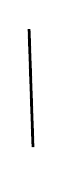
\begin{tikzpicture}\draw[line width=1pt](0,0)--(-.05,1.5);\end{tikzpicture}}

Si $A$ et $B$ sont deux schémas abéliens sur $S$, on sait en effet que $H=\underline{\operatorname{Hom}}_S(A,B)$ est représentable, et est net sur $S$, donc il suffit d'appliquer le lemme 1.

\uline{Corollaire} 3 Soit $p$ un nb premier, et soit $f:S'\mathbin{-}S$ comme dans le cor. précédent. Alors $f$ est un morphisme de descente pour la catégorie des \deleted{\unsure{gr}} schémas en groupes $p$-divisibles.

L'argument \deleted{\unsure{préc.}} du lemme 1 nous ramène à prouver l'analogue du corollaire 1, quand $X=\underline{\operatorname{Hom}}_S(A,B)$, $A,B$ deux groupes $p$-divisibles. Il faut prouver que $X$ est formellement net.
\mspage{24}
